\documentclass{standalone}
\usepackage{tikz}
\usetikzlibrary{patterns, positioning}


\begin{document}
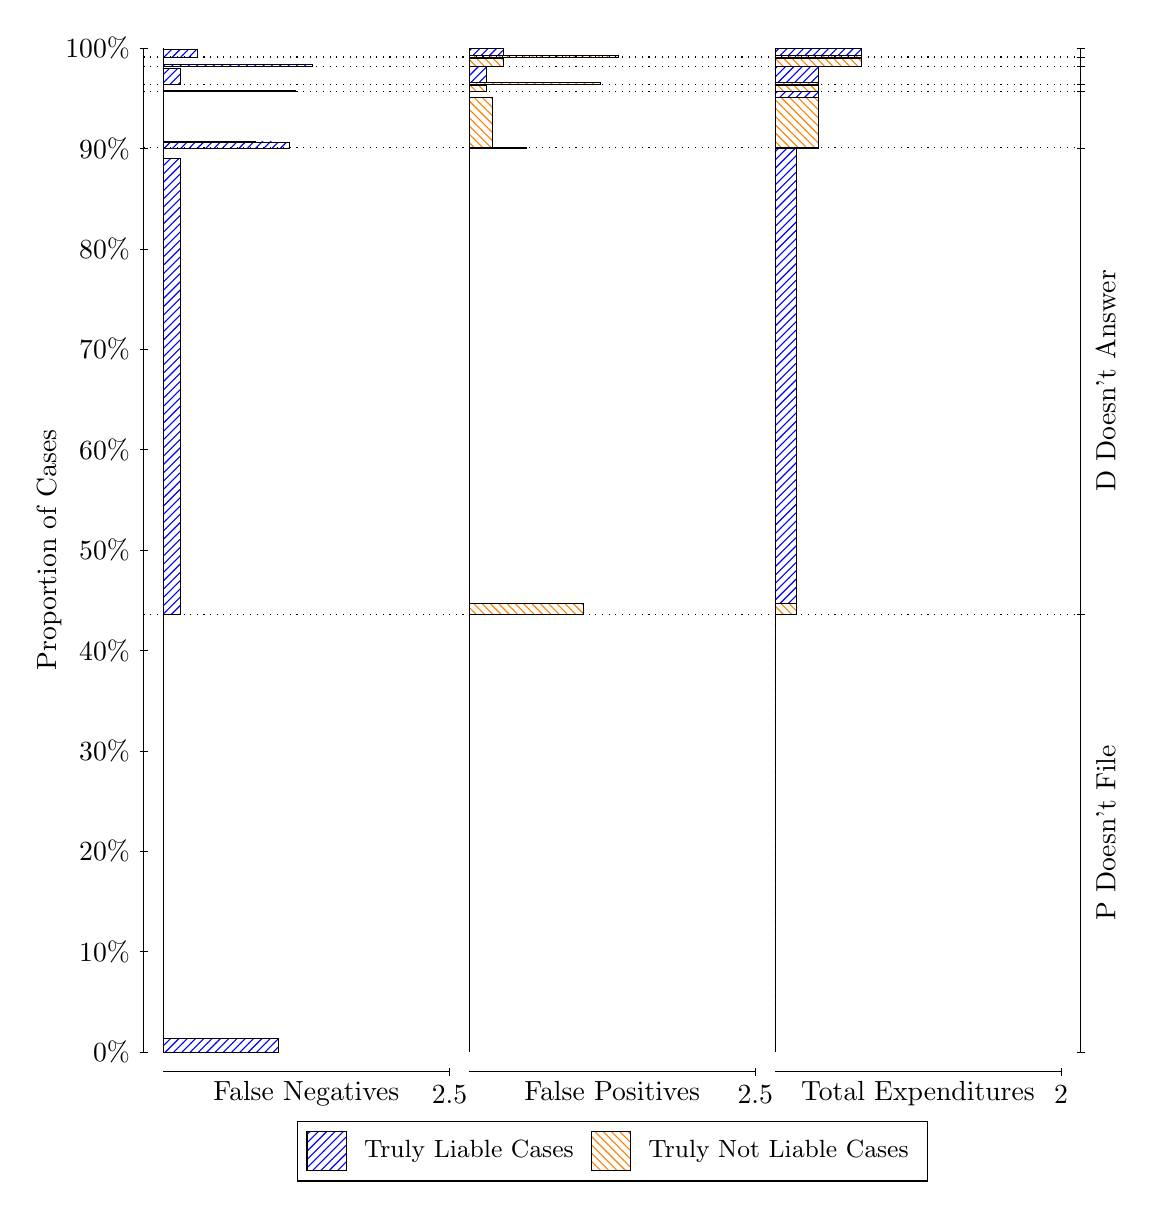
\begin{tikzpicture}
\draw[black, very thin] (1.5,1.75) -- (1.5,14.5);
\node[rotate=90, text=black, anchor=center] at (0.3, 8.125) {Proportion of Cases};
\draw[black, very thin] (1.45,1.75) -- (1.55,1.75);
\node[text=black, anchor=east] at (1.45, 1.75) {0\%};
\draw[black, very thin] (1.45,3.025) -- (1.55,3.025);
\node[text=black, anchor=east] at (1.45, 3.025) {10\%};
\draw[black, very thin] (1.45,4.3) -- (1.55,4.3);
\node[text=black, anchor=east] at (1.45, 4.3) {20\%};
\draw[black, very thin] (1.45,5.575) -- (1.55,5.575);
\node[text=black, anchor=east] at (1.45, 5.575) {30\%};
\draw[black, very thin] (1.45,6.85) -- (1.55,6.85);
\node[text=black, anchor=east] at (1.45, 6.85) {40\%};
\draw[black, very thin] (1.45,8.125) -- (1.55,8.125);
\node[text=black, anchor=east] at (1.45, 8.125) {50\%};
\draw[black, very thin] (1.45,9.4) -- (1.55,9.4);
\node[text=black, anchor=east] at (1.45, 9.4) {60\%};
\draw[black, very thin] (1.45,10.675) -- (1.55,10.675);
\node[text=black, anchor=east] at (1.45, 10.675) {70\%};
\draw[black, very thin] (1.45,11.95) -- (1.55,11.95);
\node[text=black, anchor=east] at (1.45, 11.95) {80\%};
\draw[black, very thin] (1.45,13.225) -- (1.55,13.225);
\node[text=black, anchor=east] at (1.45, 13.225) {90\%};
\draw[black, very thin] (1.45,14.5) -- (1.55,14.5);
\node[text=black, anchor=east] at (1.45, 14.5) {100\%};

\draw[black, very thin] (13.4,1.75) -- (13.4,14.5);
\draw[black, very thin] (13.35,1.75) -- (13.45,1.75);
\node[anchor=west] at (13.35, 1.75) {};
\draw[black, very thin] (13.35,7.3108) -- (13.45,7.3108);
\node[anchor=west] at (13.35, 7.3108) {};
\draw[black, very thin] (13.35,13.233) -- (13.45,13.233);
\node[anchor=west] at (13.35, 13.233) {};
\draw[black, very thin] (13.35,13.953) -- (13.45,13.953);
\node[anchor=west] at (13.35, 13.953) {};
\draw[black, very thin] (13.35,14.037) -- (13.45,14.037);
\node[anchor=west] at (13.35, 14.037) {};
\draw[black, very thin] (13.35,14.271) -- (13.45,14.271);
\node[anchor=west] at (13.35, 14.271) {};
\draw[black, very thin] (13.35,14.386) -- (13.45,14.386);
\node[anchor=west] at (13.35, 14.386) {};
\draw[black, very thin] (13.35,14.5) -- (13.45,14.5);
\node[anchor=west] at (13.35, 14.5) {};

\draw[black, very thin, pattern color=blue, pattern=north east lines] (1.75,1.75) rectangle (3.2033,1.9253);
\draw[black, very thin, pattern color=orange, pattern=north west lines] (1.75,1.9253) rectangle (1.75,7.3108);
\draw[black, very thin, pattern color=blue, pattern=north east lines] (1.75,7.3108) rectangle (1.968,13.101);
\draw[black, very thin, pattern color=orange, pattern=north west lines] (1.75,13.101) rectangle (1.75,13.233);
\draw[black, very thin, pattern color=blue, pattern=north east lines] (1.75,13.233) rectangle (3.3487,13.306);
\draw[black, very thin, pattern color=blue, pattern=north east lines] (1.75,13.306) rectangle (3.1307,13.309);
\draw[black, very thin, pattern color=blue, pattern=north east lines] (1.75,13.309) rectangle (2.9127,13.31);
\draw[black, very thin, pattern color=orange, pattern=north west lines] (1.75,13.31) rectangle (1.75,13.953);
\draw[black, very thin, pattern color=blue, pattern=north east lines] (1.75,13.953) rectangle (3.4213,13.966);
\draw[black, very thin, pattern color=orange, pattern=north west lines] (1.75,13.966) rectangle (1.75,14.037);
\draw[black, very thin, pattern color=blue, pattern=north east lines] (1.75,14.037) rectangle (1.968,14.241);
\draw[black, very thin, pattern color=orange, pattern=north west lines] (1.75,14.241) rectangle (1.75,14.271);
\draw[black, very thin, pattern color=blue, pattern=north east lines] (1.75,14.271) rectangle (3.6393,14.289);
\draw[black, very thin, pattern color=orange, pattern=north west lines] (1.75,14.289) rectangle (1.75,14.386);
\draw[black, very thin, pattern color=blue, pattern=north east lines] (1.75,14.386) rectangle (2.186,14.482);
\draw[black, very thin, pattern color=orange, pattern=north west lines] (1.75,14.482) rectangle (1.75,14.5);
\draw[black, very thin, pattern color=orange, pattern=north west lines] (5.6333,1.75) rectangle (5.6333,7.1355);
\draw[black, very thin, pattern color=blue, pattern=north east lines] (5.6333,7.1355) rectangle (5.6333,7.3108);
\draw[black, very thin, pattern color=orange, pattern=north west lines] (5.6333,7.3108) rectangle (7.0867,7.4423);
\draw[black, very thin, pattern color=blue, pattern=north east lines] (5.6333,7.4423) rectangle (5.6333,13.233);
\draw[black, very thin, pattern color=orange, pattern=north west lines] (5.6333,13.233) rectangle (6.36,13.234);
\draw[black, very thin, pattern color=orange, pattern=north west lines] (5.6333,13.234) rectangle (6.142,13.241);
\draw[black, very thin, pattern color=orange, pattern=north west lines] (5.6333,13.241) rectangle (5.924,13.875);
\draw[black, very thin, pattern color=blue, pattern=north east lines] (5.6333,13.875) rectangle (5.6333,13.953);
\draw[black, very thin, pattern color=orange, pattern=north west lines] (5.6333,13.953) rectangle (5.8513,14.024);
\draw[black, very thin, pattern color=blue, pattern=north east lines] (5.6333,14.024) rectangle (5.6333,14.037);
\draw[black, very thin, pattern color=orange, pattern=north west lines] (5.6333,14.037) rectangle (7.3047,14.067);
\draw[black, very thin, pattern color=blue, pattern=north east lines] (5.6333,14.067) rectangle (5.8513,14.271);
\draw[black, very thin, pattern color=orange, pattern=north west lines] (5.6333,14.271) rectangle (6.0693,14.368);
\draw[black, very thin, pattern color=blue, pattern=north east lines] (5.6333,14.368) rectangle (5.6333,14.386);
\draw[black, very thin, pattern color=orange, pattern=north west lines] (5.6333,14.386) rectangle (7.5227,14.403);
\draw[black, very thin, pattern color=blue, pattern=north east lines] (5.6333,14.403) rectangle (6.0693,14.5);
\draw[black, very thin, pattern color=orange, pattern=north west lines] (9.5167,1.75) rectangle (9.5167,7.1355);
\draw[black, very thin, pattern color=blue, pattern=north east lines] (9.5167,7.1355) rectangle (9.5167,7.3108);
\draw[black, very thin, pattern color=orange, pattern=north west lines] (9.5167,7.3108) rectangle (9.7892,7.4423);
\draw[black, very thin, pattern color=blue, pattern=north east lines] (9.5167,7.4423) rectangle (9.7892,13.233);
\draw[black, very thin, pattern color=orange, pattern=north west lines] (9.5167,13.233) rectangle (10.062,13.234);
\draw[black, very thin, pattern color=blue, pattern=north east lines] (9.5167,13.234) rectangle (10.062,13.235);
\draw[black, very thin, pattern color=orange, pattern=north west lines] (9.5167,13.235) rectangle (10.062,13.876);
\draw[black, very thin, pattern color=blue, pattern=north east lines] (9.5167,13.876) rectangle (10.062,13.953);
\draw[black, very thin, pattern color=orange, pattern=north west lines] (9.5167,13.953) rectangle (10.062,14.024);
\draw[black, very thin, pattern color=blue, pattern=north east lines] (9.5167,14.024) rectangle (10.062,14.037);
\draw[black, very thin, pattern color=orange, pattern=north west lines] (9.5167,14.037) rectangle (10.062,14.067);
\draw[black, very thin, pattern color=blue, pattern=north east lines] (9.5167,14.067) rectangle (10.062,14.271);
\draw[black, very thin, pattern color=orange, pattern=north west lines] (9.5167,14.271) rectangle (10.607,14.368);
\draw[black, very thin, pattern color=blue, pattern=north east lines] (9.5167,14.368) rectangle (10.607,14.386);
\draw[black, very thin, pattern color=orange, pattern=north west lines] (9.5167,14.386) rectangle (10.607,14.403);
\draw[black, very thin, pattern color=blue, pattern=north east lines] (9.5167,14.403) rectangle (10.607,14.5);
\draw[black, dotted] (1.5,7.3108) -- (13.4,7.3108);
\draw[black, dotted] (1.5,13.233) -- (13.4,13.233);
\draw[black, dotted] (1.5,13.953) -- (13.4,13.953);
\draw[black, dotted] (1.5,14.037) -- (13.4,14.037);
\draw[black, dotted] (1.5,14.271) -- (13.4,14.271);
\draw[black, dotted] (1.5,14.386) -- (13.4,14.386);
\draw[black, very thin] (1.75,1.5) -- (5.3833,1.5);
\node[text=black, anchor=north] at (3.5667, 1.5) {False Negatives};
\draw[black, very thin] (5.3833,1.45) -- (5.3833,1.55);
\node[text=black, anchor=north] at (5.3833, 1.45) {2.5};

\draw[black, very thin] (5.6333,1.5) -- (9.2667,1.5);
\node[text=black, anchor=north] at (7.45, 1.5) {False Positives};
\draw[black, very thin] (9.2667,1.45) -- (9.2667,1.55);
\node[text=black, anchor=north] at (9.2667, 1.45) {2.5};

\draw[black, very thin] (9.5167,1.5) -- (13.15,1.5);
\node[text=black, anchor=north] at (11.333, 1.5) {Total Expenditures};
\draw[black, very thin] (13.15,1.45) -- (13.15,1.55);
\node[text=black, anchor=north] at (13.15, 1.45) {2};

\node[text=black, centered, rotate=90] at (13.72, 4.5304) {P Doesn't File};
\node[text=black, centered, rotate=90] at (13.72, 10.272) {D Doesn't Answer};






\draw (7.449999999999999,1.5) node[draw=none] (baseCoordinate) {};
\begin{scope}[align=center]
        \matrix[scale=0.5, draw=black, below=0.5cm of baseCoordinate, nodes={draw}, column sep=0.1cm]{
            \node[rectangle, draw, minimum width=0.5cm, minimum height=0.5cm, pattern color=blue, pattern=north east lines] {}; &
            \node[draw=none, font=\small, text=black] (B) {Truly Liable Cases}; &
            \node[rectangle, draw, minimum width=0.5cm, minimum height=0.5cm, pattern color=orange, pattern=north west lines] {}; &
            \node[draw=none, font=\small, text=black] (B) {Truly Not Liable Cases}; \\
            };
\end{scope}

\end{tikzpicture}
\end{document}